\documentclass[12pt, a4paper, twoside]{article}
\usepackage{../labreport}
\usepackage{pdfpages}
\usepackage{circuitikz}
\usepackage{adjustbox}

\setlabreportopts[authors={Nandor Kovacs \& Céline Schuster},
    title={Glühlämpchen},
    subtitle={Aufbau von einfachen Schaltkreisen, und die Messung von Strom und Spannung},
    date={\today},
    labdate={24. März 2022}
]

\begin{document}
\maketitlepage
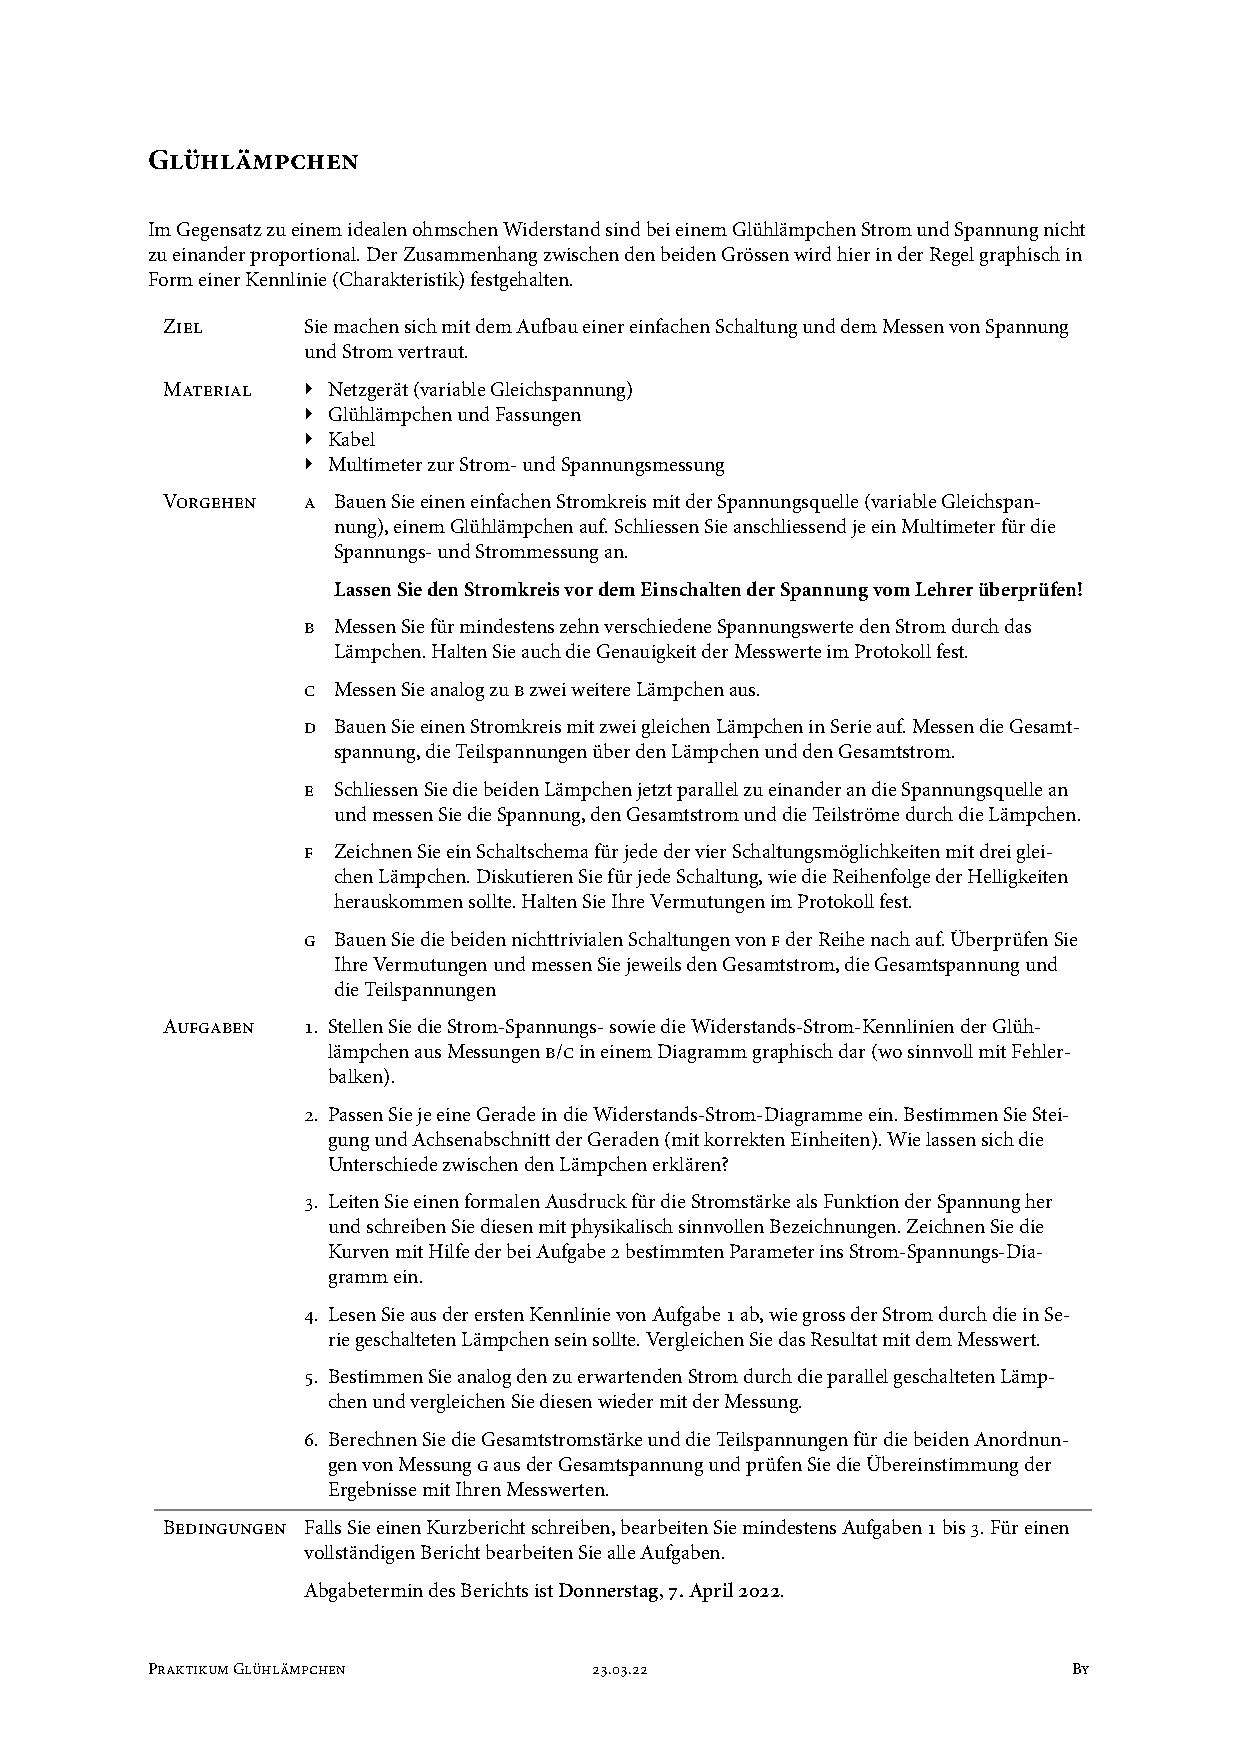
\includepdf[pages={1}]{aufgabenstellung.pdf}
\section{Einleitung}
Im Gegensatz zu herkömmlichen Widerständen ($R$) sind Strom ($I$) und Spannung ($U$) bei Glühlampen nicht proportional zueinander. Dennoch stehen diese Größen in einem gewissen Verhältnis.
In diesem Praktikum messen wir alle Werte in verschiedenen Szenarien, um ihre Beziehung herauszufinden.


\section{Theorie}
Alle unsere Schaltkreise haben drei Hauptparameter:
\begin{list}{-}{}
  \item $I$ = die Stromspannung
  \item $U$ = die Stromstärke
\end{list}

\section{Experiment}
Das Experiment bestand aus verschiedenen Stromkreisen, und Messungen an diesen Stromkreisen.
\\
\par
Für dem folgenden Stromkreis haben wir zehn Messungen gemacht für das Lämpchen 1, 5 für Lämpchen 2, und weitere 5 für Lämpchen 3.
Bei allen zehn haben wir verschiedene Spannungen angehängt.\\
\begin{align}
  \begin{circuitikz}
    \draw (0, 0.5) to[vsource] (0, 4) to[lamp] (4, 4) to[rmeterwa, t=A, l=$I_{gemessen}$] (4, 0.5) -- (0, 0.5) (0.5, 4) -- (0.5, 5) to[rmeterwa, t=V, l=$U_{gemessen}$] (3.5, 5) -- (3.5, 4);
  \end{circuitikz}
\end{align}

\datatable{c|c|c}{\csvcoli & \csvcolii & \csvcoliii}{Lämpchen 1}{$U_{start}$ & $U_{gemessen}$ & $I_{gemessen}$}{a_lamp1.csv}{a_lamp1}
\datatable{c|c|c}{\csvcoli & \csvcolii & \csvcoliii}{Lämpchen 2}{$U_{start}$ & $U_{gemessen}$ & $I_{gemessen}$}{a_lamp2.csv}{a_lamp2}
\datatable{c|c|c}{\csvcoli & \csvcolii & \csvcoliii}{Lämpchen 3}{$U_{start}$ & $U_{gemessen}$ & $I_{gemessen}$}{a_lamp2.csv}{a_lamp3}

Für diesen nächsten zwei Stromkreise haben wir je eine Messung gemacht:
\begin{align}
  \begin{circuitikz}
    \draw (0, 0) to[vsource] (0, 4) to [lamp, l=1] (2, 4) to[lamp, l=2] (4, 4) to[rmeterwa, t=A, l=$I_{gemessen}$] (4, 0) -- (0, 0) (0.25, 4) -- (0.25, 5) to[rmeterwa, t=V, l=$U_{gemessen}$] (3.75, 5) -- (3.75, 4);
  \end{circuitikz}
\end{align}

\datatable{c|c|c|c}{\csvcoli & \csvcolii & \csvcoliii & \csvcoliv}{Lämpchen 1}{$U_{gemessen}$ & $I_{total}$ & $I_{1}$ & $I_{2}$}{b_lamp1.csv}{b}



\section{Aufgaben}
\section{Fazit}
\section{Reflektion}
\section{Anhang}
Versuchsanleitung und Originalprotokoll vom \labdate
\end{document}